\section{INTRODUCCIÓN}

%\subsection{Objetivo}

El objetivo de este informe técnico es documentar el diseño e implementación de un módulo de software para configurar y controlar una placa de audio Behringer UMC204HD.  Este dispositivo forma parte del equipamiento e instrumental de la Estación Autónoma Marítima para el Monitoreo de Ruido Ambiente (EAMMRA) que se desarrolla en la División Acústica Submarina de la Dirección de Investigación de la Armada (DIIV). 

La estación EAMMRA es una boya de superficie de diseño específico para la medición de Ruido Ambiente submarino cuya concepción, diseño y fabricación se encuentran documentados en respectivos informes técnicos \citep{EAMMRA_ingConceptual}, \citep{EAMMRA_diseno} y \citep{EAMMRA_subsistemas}.  

El control de la estación en general, y la interacción con la placa en particular, se realizan con una computadora de grado industrial Kaise KBOX-S J6412. Esta computadora pertenece a la categoría de \textit{fanless embedded systems}, que son sistemas de misión específica sin partes móviles y es especialmente adecuada para aplicaciones de funcionamiento autónomo.  Cuenta con un procesador Intel Celeron J6412 de cuatro núcleos y memoria DDR4 de 16 GB \citep{kaise}, lo que le otorga al sistema una razonable capacidad de cómputo para el bajo consumo de energía que requiere la aplicación. En la figura \ref{fig:kaise} se muestra una vista frontal y trasera de la computadora y se pueden observarlas interfaces y conectores disponibles.
 
\begin{figure}[htpb]
    \centering
    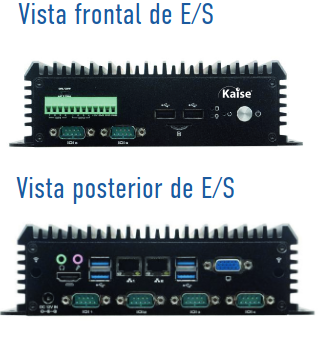
\includegraphics[width=.44\textwidth]{graficos/kaise.png}
    \caption{Vista frontal y trasera de la computadora Kaise KBOX-S J6412.}
    \label{fig:kaise}
\end{figure}


La computadora de EAMMRA corre un sistema operativo de propósitos generales, Ubuntu Server 22.04 LTS. Ubuntu Server es una distribución libre y gratuita de GNU/Linux que no requiere la compra de licencias para su uso. Este sistema operativo es reconocido por su estabilidad y seguridad, atributos esenciales para aplicaciones críticas en sistemas desatendidos como EAMMRA. Por diseño, Ubuntu Server permite una extensa personalización, con la posibilidad de realizar una instalación con los mínimos componentes necesarios, lo que permite optimizar el rendimiento general del sistema.

El módulo de software para configurar y controlar la placa de audio se implementa en Python, un lenguaje de programación interpretado y multiparadigma de alto nivel que viene integrado por defecto en las distribuciones de Ubuntu. En particular, para este módulo se utiliza Python3 que es la versión del lenguaje recomendada para proyectos nuevos, que no requieren retrocompatibilidad con componentes previos que hayan sido desarrollados en Python2.


\subsection{Herramientas de desarrollo}

Las herramientas de desarrollo de software que se utilizaron para la implementación del módulo de configuración y control permiten mejorar la calidad del código. Se entiende como código de calidad, aquel que hace lo que se supone que debe hacer, no contienen defectos ni problemas y es fácil de extender con nuevas características.

Las guías de estilo en general se utilizan para definir una forma consistente de escribir código. Si bien el estilo de codificación puede parecer una cuestión de forma, que no afecta el funcionamiento lógico del código, algunas decisiones de estilo pueden evitar errores lógicos frecuentes. Las guías definen convenciones que ayudan a mantener el código fácil de leer, mantener y extender.

Se emplearon herramientas específicas para lenguaje Python, que tienen gran difusión y aceptación en la comunidad de desarrolladores conocidas como \textit{linters}.  Estas herramientas permiten analizar el código y verificar el cumplimiento de un conjunto de reglas de mejores prácticas y buscan problemas, tanto de no conformidad con un estilo como errores de lógica.  Los defectos de lógica que se buscan son errores de código, código con resultados potencialmente no deseado y patrones de código peligroso. El uso de estas herramientas mejora la legibilidad, la mantenibilidad y la escalabilidad y hace que el código sea menos propenso a errores.   


\subsubsection{Guías de estilo para código Python - PEP-8 y PEP-257}

Para la escritura del código Python del módulo de configuración y control se adopta la guía de estilo \textit{Python Enhancement Proposal} 8 (PEP-8). Su objetivo principal es mejorar la legibilidad y coherencia del código Python y tiene amplia aceptación dentro de la comunidad de desarrolladores de este lenguaje. La guía fue escrita en 2001 por Guido van Rossum, Barry Warsaw y Nick Coghlan, basándose en las mejores prácticas existentes y las recomendaciones de la comunidad \citep{pep8}. Esta guía fomenta buenas prácticas y técnicas que pueden ayudar a evitar errores comunes.

La guía cubre varios aspectos de la codificación, que incluyen:

\begin{itemize}
	\item Formato del código: indentación, uso de espacios en blanco, longitud de las líneas, etc.
	\item Convenciones de nomenclatura: cómo nombrar variables, funciones, clases, módulos, etc.
	\item Principios de codificación: recomendaciones sobre cómo escribir expresiones y declaraciones de manera clara.
	\item Comentarios: cuándo y cómo usar comentarios para mejorar la legibilidad del código.
\end{itemize}

Asimismo, se utiliza la convención \textit{Python Enhancement Proposal} 257, (PEP-257).  Esta convención define el formato y estilo para la documentación, también llamada \textit{Python's docstrings} que aplica a módulos, clases, funciones y métodos \citep{pep257}.  Adicionalmente, si los \textit{docstring} se escriben en forma consistente, exiten herramientas capaces de generar documentación directamente del código.  Esto permite mantener más fácilmente la documentación actualizada dentro del mismo código.

Existen herramientas de desarrollo como pycodestyle y pydocstyle que verifican el estilo y ayudan a asegurar que el código cumpla con las convenciones de PEP-8 y PEP-257, respectivamente.  Estas herramientas pertenecen a la categoría de linters de estilo y en algunos casos vienen integrados dentro de otros linters como Flake8 o Pylama.

\subsubsection{Style guide enforcement - Flake8}

Flake8 es una herramienta que permite imponer y hacer cumplir las directivas de la guía de estilo PEP-8 y pertenece a la familia de programas tipo \textit{lint} que trabajan analizando el código fuente para verificar el cumplimiento de un conjunto definido de reglas. Esta herramienta puede señalar errores de programación, \textit{bugs}, errores de estilo y construcciones sospechosas. Es altamente configurable, y permite a los desarrolladores ajustar las reglas y la severidad de las advertencias según las necesidades específicas de su proyecto \citep{flake8}.

Para instalar flake8 para la versión por defecto de Python:

\begin{lstlisting}[language=bash]
python -m pip install flake8
\end{lstlisting}

Para utilizar flake8, se deben ejecutar los siguientes comando desde una terminal interactiva:

\begin{lstlisting}[language=bash]
flake8 path/to/code/to/check.py
# or
flake8 path/to/code/
\end{lstlisting}

%\clearpage

A su vez, se puede seleccionar una regla específica para ejecutar o ignorar:

\begin{lstlisting}[language={python}]
flake8 --select E123,W503 path/to/code/
# or
flake8 --extend-ignore E203,W234 path/to/code/
\end{lstlisting}

El listado completo de códigos de error y su significado puede encontrarse en el sitio weboficial de la herramienta, \url{http://flake8.pycqa.org/en/latest/user/error-codes.html}.

\subsubsection{Analizador estático - Pylint}
Pylint es una herramienta de análisis estático de código para Python que busca errores de programación, ayuda a hacer cumplir un estándar de codificación y busca ``malos olores'' en el código (\textit{code smells}). Utiliza diferentes técnicas para analizar el código fuente y puede identificar problemas o patrones de codificación problemáticos que podrían llevar a errores o a un código difícil de mantener o leer \citep{pylint}. 

Las características principales de Pylint incluyen:

\begin{itemize}
    \item Chequeo de errores: puede detectar errores que podrían hacer que el código falle en tiempo de ejecución, como llamadas a funciones no definidas, uso de variables antes de su definición, etc.
    \item Estándares de codificación: Pylint puede asegurar de que el código siga un estándar de codificación particular, como PEP-8.
    \item Refactorización de código: sugiere lugares donde el código podría ser refactorizado para mejorar la legibilidad o la eficiencia.
    \item Detección de código duplicado: puede identificar bloques de código duplicados que podrían ser simplificados o extraídos en una función común.
    \item Chequeo de tipos: aunque Python es un lenguaje dinámicamente tipado, Pylint puede realizar algunas comprobaciones de tipos para identificar posibles problemas.
\end{itemize}

Para instalar pylint para la versión por defecto de Python:

\begin{lstlisting}[language=bash]
python -m pip install pylint
\end{lstlisting}

Para utilizar pylint, se debe ejecutar el siguiente comando:

\begin{lstlisting}[language=bash]
pylint [options] modules_or_packages
\end{lstlisting}

%\begingroup %inexplicablemente esto hace que la url fittee bien 
%\sloppy
%
%\endgroup

Pylint agrega un prefijo a cada una de las áreas problemáticas con una R, C, W, E o F, que significan:

\begin{itemize}
    \item \textbf{R}efactorizar por una violación de la métrica de ``buena práctica''.
    \item \textbf{C}onvención por violación del estándar de codificación.
    \item \textbf{W}arning (Advertencia) por problemas estilísticos o problemas de programación menores.
    \item \textbf{E}rror por problemas importantes de programación (es decir, muy probablemente un bug).
    \item \textbf{F}atal por errores que impidieron el procesamiento adicional.
\end{itemize}

La lista completa de mensajes y su significado puede encontrarse en el sitio web oficial de la herramienta, donde se encuentran agrupados por categoría o área problemática.  La url es: \small{\url{https://pylint.pycqa.org/en/latest/user_guide/messages/messages_overview.html}}.

\subsubsection{Formato automático - Black}

Black es una herramienta de formateo de código para Python conocida por su enfoque en la simplicidad y la uniformidad. A menudo se le llama ``el formateador de código sin compromisos'' debido a su filosofía de tener una sola forma estandarizada y automatizada de formatear el código Python. Esto contrasta con otras herramientas de formateo que pueden permitir una mayor configuración o variaciones en el estilo de codificación \citep{black}.

Algunas características clave de Black incluyen:

\begin{itemize}
    \item Automatización: Black reformatea todo el archivo de código con solo un comando, sin necesidad de ajustes manuales.
    \item Consistencia: aplica un estilo consistente en todos los proyectos de Python al seguir un conjunto de reglas predefinido, lo que ayuda a mejorar la legibilidad y reducir el tiempo dedicado a discutir sobre estilos de codificación en revisiones de código.
    \item Integración fácil: puede integrarse fácilmente con editores de texto y entornos de desarrollo integrados (IDEs), así como con sistemas de integración continua/entrega continua (CI/CD).
    \item Seguridad: está diseñado para realizar cambios en el código que no afecten su comportamiento, lo que lo hace seguro para usar en proyectos grandes y complejos.
\end{itemize}

Al tener el código un formato unificado entre los distintos desarrolladores, las revisiones de código, especialmente bajo control de versiones, se pueden hacer más rápidamente debido a que los \textit{diffs }entre versiones son lo más pequeños posible.  Black es un formateador de código PEP-8 compatible.

Para instalar Black, se debe ejecutar el siguiente comando en una terminal:

\begin{lstlisting}[language=bash]
python pip install black
\end{lstlisting}

Para utilizar Black, se debe ejecutar el siguiente comando:

\begin{lstlisting}[language=bash]
black modules_or_packages
\end{lstlisting}

\subsubsection{Entorno de Desarrollo Integrado - Visual Studio Code}

Visual Studio Code, disponible en \url{https://code.visualstudio.com/}, es un editor de código fuente de código abierto que soporta múltiples lenguajes de programación. Destaca por su flexibilidad y capacidad de personalización. Permite integrar extensiones que amplían sus funcionalidades. Entre sus características se encuentran el soporte para depuración integrada, control de versiones con Git y herramientas de autocompletado. También ofrece una interfaz de usuario intuitiva y un sistema de gestión de proyectos eficiente. VSCode es compatible con Windows, macOS y GNU/Linux.

Existen múltiples extensiones disponibles para Python. Entre las más destacadas se encuentran el plugin \texttt{Python}, que proporciona soporte para depuración, ejecución de código, y autocompletado de código Python, y \texttt{Pylance}, que ofrece características adicionales como análisis estático de código y autocompletado inteligente.

La extensión Remote - SSH de Visual Studio Code permite utilizar cualquier máquina remota con un servidor SSH como entorno de desarrollo. Esto facilita el desarrollo y la resolución de problemas en una amplia variedad de situaciones. Mediante esta extensión, es posible desarrollar en el mismo sistema operativo al que se desplegará el software o emplear hardware más grande, rápido o especializado que el de la máquina local.

Una de las ventajas de esta extensión es la capacidad de cambiar rápidamente entre diferentes entornos de desarrollo remotos, lo que permite realizar actualizaciones de manera segura sin riesgo de afectar la máquina local. Además, proporciona acceso a un entorno de desarrollo ya existente desde varias máquinas o ubicaciones, lo que aumenta la flexibilidad del proceso de desarrollo.

Esta extensión resulta útil también para depurar aplicaciones que se ejecutan en otros lugares. No es necesario tener el código fuente en la máquina local para aprovechar estas ventajas, ya que la extensión ejecuta comandos y otras extensiones directamente en la máquina remota. Es posible abrir cualquier carpeta en la máquina remota y trabajar con ella de la misma forma que si estuviera en la máquina local.

\clearpage
\section{PLACA DE AUDIO BEHRINGER UMC204HD}

La Behringer UMC204HD es una interfaz de audio de alta calidad diseñada para la captura y procesamiento de señales de audio. Esta interfaz es compatible con sistemas operativos modernos Windows y GNU/Linux y se conecta a través de un puerto USB 2.0. Su capacidad para trabajar con alta resolución vertical y elevadas tasas de muestreo la convierte en una herramienta útil para una variedad de aplicaciones profesionales en el ámbito del análisis de señales. En la figura \ref{fig:placa} se puede apreciar una vista frontal y trasera de la interfaz de audio UMC204HD.

La Behringer UMC204HD ofrece una resolución vertical de 24 bits, lo que permite una captura precisa y detallada de las señales de entrada. Esta alta resolución es esencial para la adquisición de datos en aplicaciones que requieren una representación fiel de las variaciones más pequeñas en la señal, como es el caso de señales adquieridas con hidrófonos.

La interfaz tiene una tasa de muestreo de hasta 192 kHz, lo que le permite capturar señales con una adecuada resolución temporal. Esta alta tasa de muestreo es crucial para evitar el fonómeno de \textit{aliasing} y para asegurar que las señales con contenido espectral en altas frecuencias, como las señales provenientes de los hidrófonos, se capturen adecuadamente.  Asimismo, la interface UMC204HD se caracteriza por tener bajo nivel de ruido propio. 

\vspace{10px}
\begin{figure}[ht]
    \centering
    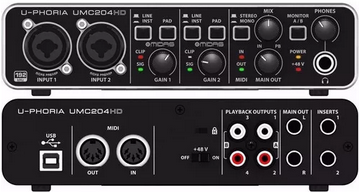
\includegraphics[width=.5\textwidth]{graficos/behringer.png}
    \caption[]{Vista frontal y trasera de la interface de audio Behringer UMC204HD.}
    \label{fig:placa}
\end{figure}

\clearpage
\section{DISEÑO E IMPLEMENTACIÓN }

\subsection{Descripción general del módulo}

El módulo \texttt{BehringerHandler} fue desarrollado en Python con el objetivo de controlar una interfaz de audio USB marca Behringer de forma programática. Permite su inicialización, apertura de flujos de entrada, grabación asincrónica y gestión completa de recursos. Está pensado para ser utilizado en sistemas de adquisición acústica en tiempo real, y su diseño modular facilita su integración en arquitecturas mayores, como estaciones de monitoreo o sistemas embebidos.

El funcionamiento interno del módulo se apoya en varias bibliotecas estándar y externas. Utiliza \texttt{pyaudio} para el acceso de bajo nivel al hardware de audio, \texttt{wave} para la escritura de los datos capturados en formato WAV, \texttt{threading} para realizar la grabación en paralelo al hilo principal y \texttt{queue} para sincronizar los datos entre procesos. Además, se emplean \texttt{logging} para la trazabilidad de eventos, \texttt{datetime} para la generación de nombres de archivo basados en marca temporal y \texttt{os} para la gestión del entorno de ejecución y rutas de archivo. Esta combinación de módulos permite una operación robusta, escalable y fácilmente depurable.

La biblioteca \texttt{logging} de Python se utiliza para generar registros estructurados durante la ejecución del código, y permite monitorear el estado del sistema, detectar errores y realizar trazabilidad de eventos. En el módulo \texttt{BehringerHandler}, se implementa un sistema de log dual que escribe tanto en consola como en un archivo de texto (\texttt{behringer\_handler.log}). Este sistema utiliza formatos personalizados con marcas de tiempo y niveles de severidad (INFO, WARNING, ERROR), lo que facilita el diagnóstico en tiempo real y la revisión posterior del funcionamiento del sistema. La inclusión de \texttt{logging} mejora la mantenibilidad y confiabilidad del software, especialmente en entornos donde no hay interacción directa con el usuario.

La biblioteca \texttt{PyAudio} proporciona una interfaz en Python para interactuar con PortAudio, una biblioteca de código abierto para la captura y reproducción de audio en tiempo real. Este paquete permite abrir flujos de entrada o salida de audio con parámetros configurables como tasa de muestreo, formato, número de canales y tamaño de buffer. En el caso de \texttt{BehringerHandler}, \texttt{PyAudio} es utilizado para detectar dispositivos de audio disponibles, abrir un flujo de entrada en formato \texttt{paInt24} y capturar señales a alta resolución (192 kHz, 2 canales). Gracias a su capacidad para operar en modo no bloqueante mediante callbacks, \texttt{PyAudio} permite implementar grabaciones asincrónicas eficientes, fundamentales para aplicaciones de adquisición continua o en tiempo real.

La biblioteca estándar \texttt{wave} de Python permite la manipulación de archivos de audio en formato WAV (RIFF). Proporciona una interfaz sencilla para la escritura y lectura de audio en formato PCM (Pulse Code Modulation), y permite definir parámetros como la cantidad de canales, la tasa de muestreo y la resolución en bits. En el módulo \texttt{BehringerHandler}, \texttt{wave} se utiliza para almacenar las grabaciones capturadas por el stream de PyAudio en archivos de alta calidad de 24 bits. La escritura se realiza en tiempo real desde un hilo separado, para asegurar la integridad de los datos y su disponibilidad inmediata en disco para posteriores análisis.

La biblioteca \texttt{threading} proporciona soporte para la ejecución concurrente de código mediante la creación y gestión de hilos de ejecución. En \texttt{BehringerHandler}, se utiliza para realizar la escritura de audio en disco de forma asincrónica, separando la captura en tiempo real del procesamiento de los datos. Esto permite que el flujo principal de adquisición no se vea interrumpido por operaciones de entrada/salida, lo que mejora el rendimiento y evita pérdidas de datos. El uso de \texttt{threading} resulta esencial para garantizar grabaciones continuas y confiables, especialmente en sistemas que requieren alta tasa de muestreo o baja latencia.

La biblioteca \texttt{queue} proporciona una estructura de datos segura para comunicación entre hilos en entornos multithreading. En el módulo \texttt{BehringerHandler}, se utiliza una instancia de \texttt{Queue} para almacenar de forma temporal los bloques de audio recibidos por el callback del stream de PyAudio. Esta cola permite desacoplar la adquisición de datos (en tiempo real) de la escritura en disco, evitando pérdidas o bloqueos por operaciones lentas de entrada/salida. El uso de \texttt{queue} garantiza una sincronización segura y eficiente entre el hilo de captura y el hilo de grabación.

La biblioteca estándar \texttt{datetime} permite manipular fechas y horas de manera precisa y flexible. En el módulo  \texttt{BehringerHandler}, se utiliza para generar marcas de tiempo en el momento de iniciar una grabación, lo que permite construir nombres de archivo únicos con el formato \texttt{YYYYMMDD\_HHMMSS}. Esta práctica facilita la organización de las grabaciones, evita sobreescrituras accidentales y proporciona una trazabilidad temporal inmediata. El uso de \texttt{datetime} también permite registrar eventos en los logs con exactitud temporal.

La biblioteca estándar \texttt{os} proporciona funciones para interactuar con el sistema operativo de forma portable. En el módulo \texttt{BehringerHandler}, se utiliza para obtener la ruta absoluta del script en ejecución, crear subdirectorios (como \texttt{recordings} para guardar archivos de audio) y construir rutas de forma segura e independiente del sistema operativo.  El uso de \texttt{os} es esencial para garantizar la correcta gestión de archivos y configuraciones en distintos entornos de ejecución.

\subsection{Dependencias y gestión del entorno}

La lista completa de dependencias necesarias para ejecutar el módulo \texttt{BehringerHandler} se encuentra documentada en el archivo \texttt{requirements.txt}. Este archivo fue generado utilizando el comando \texttt{pip freeze > requirements.txt} desde un entorno virtual de Python configurado específicamente para este proyecto. La utilización de entornos virtuales permite aislar las versiones de los paquetes, asegurando la reproducibilidad del entorno de ejecución.

Para reconstruir el entorno en una nueva máquina o entorno limpio, se recomienda crear un entorno virtual (por ejemplo, mediante \texttt{python -m venv venv}) y luego instalar todas las dependencias mediante el comando \texttt{pip install -r requirements.txt}. Esto garantiza que las versiones exactas utilizadas durante el desarrollo serán replicadas, y permite reducir los  errores por incompatibilidades entre bibliotecas.

A continuación, se presenta la lista de dependencias incluidas en \texttt{requirements.txt}:

\begin{verbatim}
contourpy==1.3.1
cycler==0.12.1
fonttools==4.56.0
iniconfig==2.1.0
kiwisolver==1.4.8
matplotlib==3.10.1
numpy==2.2.3
packaging==24.2
pillow==11.1.0
pluggy==1.5.0
PyAudio==0.2.14
pyparsing==3.2.1
pytest==8.3.5
python-dateutil==2.9.0.post0
schedule==1.2.2
six==1.17.0
\end{verbatim}


\subsection{Arquitectura del módulo}

El diseño está centrado en la clase \texttt{BehringerHandler}, que actúa como fachada para todas las operaciones necesarias. La arquitectura sigue una lógica secuencial:

\begin{enumerate}
    \item Inicialización del entorno (\texttt{init}): escanea los dispositivos de audio y selecciona automáticamente el que corresponde a Behringer.
    \item Apertura del flujo de entrada (\texttt{open}).
    \item Grabación asincrónica (\texttt{record} y \texttt{\_write\_audio}) mediante un hilo dedicado y una cola de datos.
    \item Cierre y liberación de recursos (\texttt{stop\_recording}, \texttt{close}, \texttt{deinit}).
\end{enumerate}

En la figura \ref{fig:workflow} se presenta un diagrama de flujo general con los bloques principales y la secuencia lógica de ejecución del módulo Beheringer\_Handler.

\begin{figure}[htpb]
    \centering
    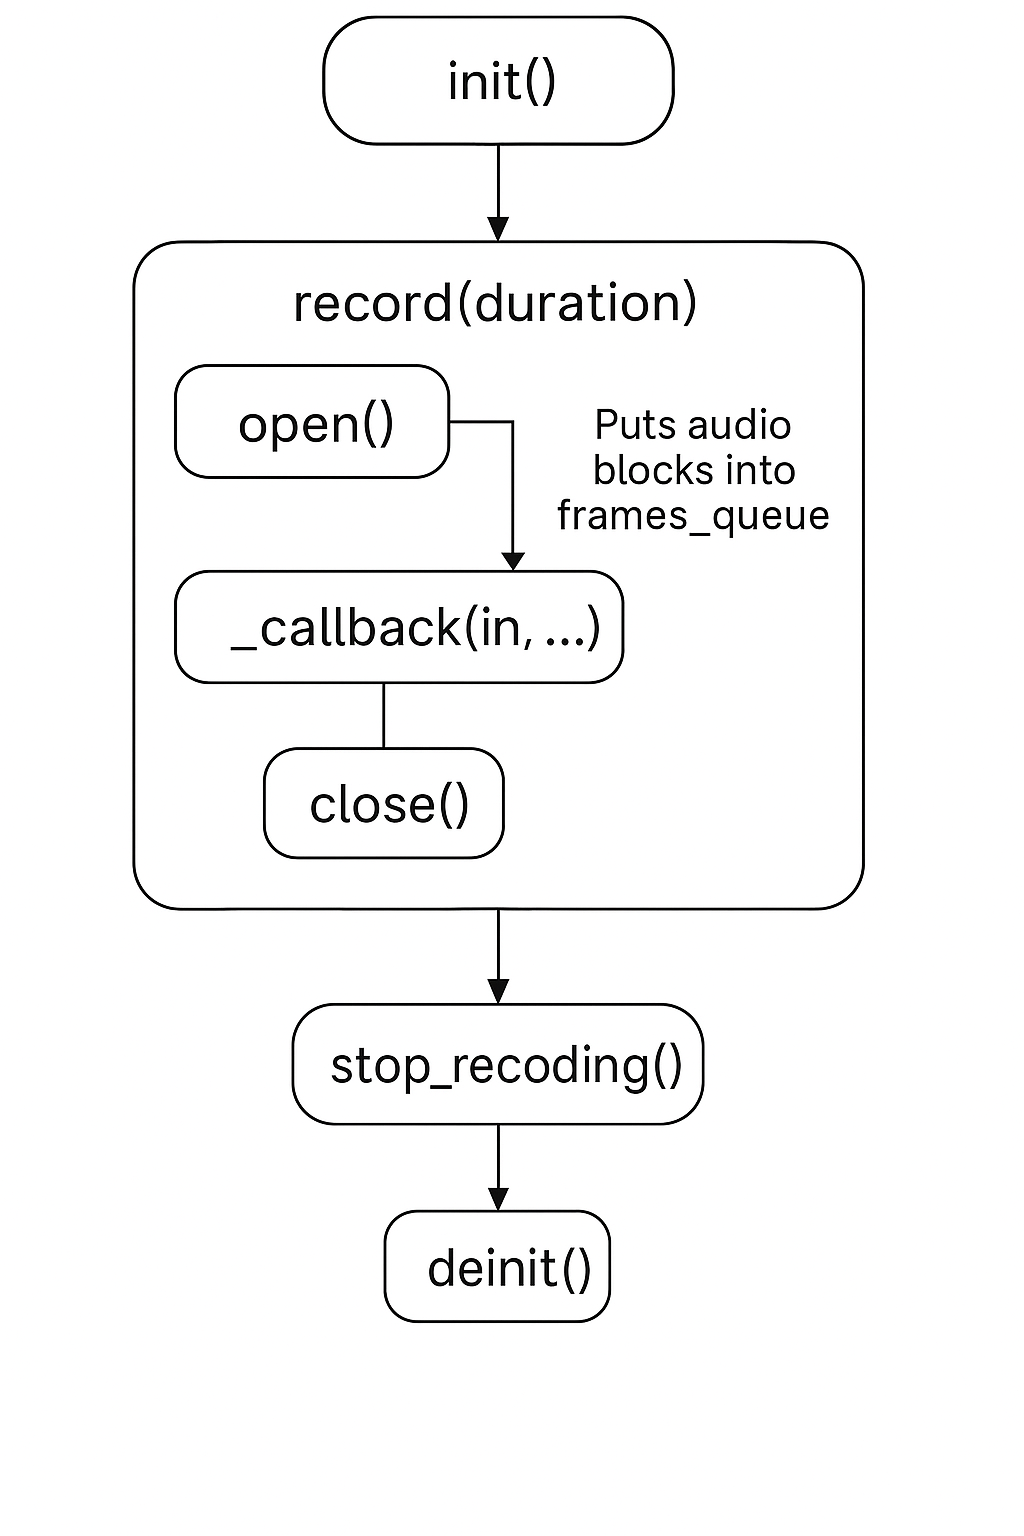
\includegraphics[width=0.6\textwidth]{graficos/workflow.png}
    \caption{Diagrama de flujo de funcionamiento del módulo \texttt{BehringerHandler}}
    \label{fig:workflow}
\end{figure}

Durante la ejecución, los eventos relevantes se registran tanto en consola como el archivo con extensión .log.

\subsection{Uso del módulo}

El flujo de uso del módulo es el siguiente:

\begin{verbatim}
from behringer_handler import BehringerHandler

handler = BehringerHandler()
handler.init()
handler.record(duration=10)  # graba 10 segundos de audio
handler.stop_recording()
handler.deinit()
\end{verbatim}

\subsection{Descripción de la clase y sus métodos}

\texttt{BehringerHandler} extiende de \texttt{BaseHandler} e implementa los métodos clave para el manejo del dispositivo. La utilización de una clase base común responde a una estrategia de diseño orientada a la modularidad y escalabilidad del sistema EAMRRA, donde múltiples módulos de adquisición o control comparten una estructura funcional similar. 

La clase \texttt{BaseHandler} actúa como plantilla abstracta, y define una interfaz mínima que obliga a los módulos derivados a implementar ciertos métodos esenciales, como \texttt{init}, \texttt{deinit}, \texttt{open} y \texttt{close}. Esta decisión asegura una simetría en la arquitectura del sistema, facilita el mantenimiento y permite la integración homogénea de nuevos módulos en el futuro. Además, permite aplicar patrones de programación como la inversión de dependencias, delegando a cada módulo el detalle de implementación mientras se conserva una estructura común y predecible.

A continuación se describen los métodos principales de la clase \texttt{BehringerHandler}:

\subsubsection*{\texttt{\_\_init\_\_}}

Constructor de la clase. Inicializa atributos, crea el logger y configura los manejadores de archivo y consola.

\subsubsection*{\texttt{init()}}

Escanea los dispositivos de audio disponibles con PyAudio. Si encuentra uno con el nombre \texttt{Behringer} o que incluya \texttt{USB} y tenga canales de entrada, lo selecciona y guarda su índice.

\subsubsection*{\texttt{open()}}

Abre un stream de entrada en modo no bloqueante para el dispositivo detectado, utilizando formato \texttt{paInt24}, dos canales, y frecuencia de muestreo de 192 kHz. Registra advertencias si el dispositivo no está inicializado.

\subsubsection*{\texttt{\_callback(in\_data, frame\_count, time\_info, status)}}

Función callback del stream. Si la grabación está activa, coloca los datos de entrada en una cola de frames. Si no, retorna \texttt{paComplete}.

\subsubsection*{\texttt{record(duration)}}

Inicia una grabación de duración determinada (en segundos). Crea un hilo que ejecuta \texttt{\_write\_audio}, abre el stream e inicia la adquisición. El archivo de salida se guarda con nombre basado en fecha y hora en la carpeta \texttt{recordings}.

\subsubsection*{\texttt{\_write\_audio()}}

Hilo que extrae datos de la cola y los escribe dinámicamente en un archivo WAV. Utiliza \texttt{wave} para manejar el formato y guarda las grabaciones en disco hasta que se completa el tiempo solicitado.

\subsubsection*{\texttt{stop\_recording()}}

Detiene la grabación, cierra el hilo de escritura y registra el evento.

\subsubsection*{\texttt{deinit()}}

Libera el objeto PyAudio, permite reinicializar el sistema si se vuelve a ejecutar \texttt{init()}.

\subsubsection*{\texttt{close()}}

Detiene y cierra el stream de audio si está activo. Libera la referencia.

\subsection{Diagrama de flujo del módulo}




\clearpage
\section{PRUEBAS Y ENSAYOS}

\clearpage
\section{CONCLUSIONES}

%